% ============================================================================
% EDC Neutron-Proton Mass Difference Derivation
% Companion G to Paper 3 (NJSR Edition)
% Version: 2.1 | Date: 2026-01-19
% Build: XeLaTeX (Unicode)
% ============================================================================

\documentclass[11pt,a4paper]{article}

% Packages
\usepackage{fontspec}
\usepackage{amsmath,amssymb,amsthm}
\usepackage{physics}
\usepackage{geometry}

% FONTS (TeX Gyre Termes = Times-like with full OpenType support)
\IfFontExistsTF{TeX Gyre Termes}{%
  \setmainfont{TeX Gyre Termes}
  \setsansfont{TeX Gyre Heros}
}{%
  \setmainfont{Times New Roman}[Ligatures=TeX]
  \setsansfont{Helvetica}
}
\usepackage[colorlinks=true,linkcolor=blue,citecolor=blue,urlcolor=blue,pdfborder={0 0 0}]{hyperref}
\usepackage{booktabs}
\usepackage{enumitem}
\usepackage{tikz}
\usetikzlibrary{calc,arrows.meta}
\usepackage{gensymb}
\usepackage{xcolor}
\usepackage{tcolorbox}

\geometry{margin=2.5cm}

% ============================================================================
% EPISTEMIC TAG COLORS
% ============================================================================
\definecolor{tagDer}{RGB}{0,100,0}      % Green - Derived
\definecolor{tagDc}{RGB}{0,80,160}      % Blue - Deduced/Constrained
\definecolor{tagCal}{RGB}{0,128,128}    % Teal - Calibrated
\definecolor{tagI}{RGB}{100,0,100}      % Purple - Identified
\definecolor{tagP}{RGB}{150,0,0}        % Red - Postulated
\definecolor{tagOpen}{RGB}{200,0,0}     % Bright red - Open
\definecolor{tagBL}{RGB}{128,64,0}      % Brown - Baseline

% ============================================================================
% EPISTEMIC TAG COMMANDS
% ============================================================================
\newcommand{\tagDer}{\textcolor{tagDer}{\textbf{[Der]}}}
\newcommand{\tagDc}{\textcolor{tagDc}{\textbf{[Dc]}}}
\newcommand{\tagCal}{\textcolor{tagCal}{\textbf{[Cal]}}}
\newcommand{\tagI}{\textcolor{tagI}{\textbf{[I]}}}
\newcommand{\tagP}{\textcolor{tagP}{\textbf{[P]}}}
\newcommand{\tagOpen}{\textcolor{tagOpen}{\textbf{[OPEN]}}}
\newcommand{\tagBL}{\textcolor{tagBL}{\textbf{[BL]}}}

% ============================================================================
% THEOREM ENVIRONMENTS
% ============================================================================
\newtheorem{theorem}{Theorem}[section]
\newtheorem{lemma}[theorem]{Lemma}
\newtheorem{proposition}[theorem]{Proposition}
\newtheorem{corollary}[theorem]{Corollary}
\newtheorem{definition}[theorem]{Definition}
\newtheorem{postulate}{Postulate}

\theoremstyle{remark}
\newtheorem{remark}{Remark}[section]

% ============================================================================
% CUSTOM COMMANDS
% ============================================================================
\newcommand{\Rxi}{R_\xi}
\newcommand{\re}{r_e}
\newcommand{\Ztri}{\mathbb{Z}_3}
\newcommand{\Ztwo}{\mathbb{Z}_2}
\newcommand{\Zsix}{\mathbb{Z}_6}
\newcommand{\Mfive}{M_5}
\newcommand{\Mfour}{M_4}
\newcommand{\Sone}{S^1}

% ============================================================================
% TITLE
% ============================================================================
\title{\textbf{Neutron-Proton Mass Difference from 5D Y-Junction Topology}\\[0.5em]
\large Consolidated Mathematical Derivation\\[0.3em]
\normalsize (Companion G to Paper~3: NJSR Edition)}
\author{Igor Gr\v{c}man}
\date{January 2026\\[0.5em]
\small Repository: \href{https://github.com/igorgrcman/elastic-diffusive-cosmology}{github.com/igorgrcman/elastic-diffusive-cosmology}\\[0.2em]
\footnotesize (Public artifacts for this paper are in the \texttt{edc\_papers} folder.)}

\begin{document}

\maketitle

% ============================================================================
% RELATED DOCUMENTS
% ============================================================================
\begin{center}
\small\textbf{Related Documents:}\\[0.1cm]
\footnotesize
\textbf{Companions:}\\
\end{center}

% ============================================================================
% TAGGING STANDARD BOX
% ============================================================================
\begin{tcolorbox}[colback=green!5,colframe=green!40!black,title=\textbf{Epistemic Tagging Standard}]
All claims carry explicit tags indicating derivation status:
\begin{center}
\renewcommand{\arraystretch}{1.2}
\begin{tabular}{@{}cl@{}}
\toprule
\textbf{Tag} & \textbf{Meaning} \\
\midrule
\tagDer{} & Derived: explicit mathematical derivation from stated postulates \\
\tagDc{} & Deduced/Constrained: follows from assumptions with explicit ansatz \\
\tagCal{} & Calibrated: parameter fitted to match experimental value \\
\tagI{} & Identified: pattern matching without full derivation \\
\tagP{} & Postulated: foundational assumption; not derived \\
\tagOpen{} & Open: known gap; future work needed \\
\tagBL{} & Baseline: external empirical input (CODATA, PDG, SM) \\
\bottomrule
\end{tabular}
\end{center}
\end{tcolorbox}

% ============================================================================
% ABSTRACT
% ============================================================================
\begin{abstract}
\noindent
This companion paper presents the derivation of the neutron-proton mass difference $\Delta m = m_n - m_p = 1.293$~MeV \tagBL{} from 5D Y-junction topology in Elastic Diffusive Cosmology (EDC).

\textbf{What this paper does:} Establishes (1) $\Zsix = \Ztri \times \Ztwo$ symmetry from ring oscillation topology \tagDc, (2) the asymmetry parameter $q = 1/3$ from the half-Steiner configuration at $\delta\theta = 60\degree$ \tagDer, (3) the prefactor $1/6$ from brane embedding geometry \tagDc, and (4) connections to SU(3) color structure \tagI. The result matches experiment to 0.6\% accuracy.

\textbf{What this paper does NOT do:} Derive the energy scale $\sigma\re^2$ from first principles \tagOpen, or prove the claim constitutes a genuine prediction rather than a calibrated consistency check.

\textbf{Calibration boundary:} Two scale inputs enter this calculation:
\begin{itemize}[nosep,leftmargin=*]
    \item $V_3 = -0.65$~MeV \tagCal{} --- tuned to match $\Delta m$
    \item $\sigma\re^2 = 70$~MeV \tagBL{} --- external nuclear-scale input (not fitted here)
\end{itemize}
The geometric factors ($q = 1/3$, prefactor $1/6$) are not fitted. This paper is a \textbf{consistency check}, not an ab initio prediction.

\textbf{Units convention:} We use natural units $c = \hbar = 1$. All energies are in MeV; mass $m$ and energy $E$ are interchangeable (i.e., $\Delta m = 1.293$~MeV means $\Delta E = 1.293$~MeV).
\end{abstract}

\tableofcontents

% ============================================================================
\section{Introduction and Setup}
% ============================================================================

\subsection{The Y-Junction Structure}

\begin{postulate}[Y-Junction Topology] \tagP
\label{post:y-junction}
In EDC, baryons are represented as Y-junctions---three flux tubes meeting at a common vertex embedded in a 5D manifold $\Mfive = \Mfour \times \Sone_\xi$.
\end{postulate}

\begin{remark}[Foundation in Companion~F]
\textbf{Companion~F} (``Proton as 5D Junction: Variational Foundation'') derives the $120\degree$ angle geometry from energy minimization: equal-tension arms satisfy $\sum_i \sigma\hat{t}_i = 0$, which forces Steiner angles \tagDer{}. This companion builds on that foundation to analyze symmetry breaking.
\end{remark}

\begin{definition}[Y-Junction]
A Y-junction is a 1-dimensional defect where three flux tubes (strings) meet at a vertex $V$. Each arm $i \in \{1,2,3\}$ carries:
\begin{itemize}
    \item Direction vector $\hat{e}_i$ in the transverse plane
    \item Winding number $W_i$ around the compact dimension $S^1_\xi$
    \item Tension $\tau = \sigma \cdot a$ where $\sigma$ is membrane tension and $a$ is string cross-section
\end{itemize}
\end{definition}

\subsection{Steiner Configuration}

\begin{definition}[Steiner Point]
The Steiner configuration minimizes total string length for fixed endpoints. At the Steiner point:
\begin{equation}
\theta_{12} = \theta_{23} = \theta_{31} = 120\degree
\end{equation}
where $\theta_{ij}$ is the angle between arms $i$ and $j$.
\end{definition}

\subsection{O(2) Transverse Sector}

The junction vertex can move in the transverse plane perpendicular to the brane, parameterized by an angle $\theta \in [0, 2\pi)$. This defines the ``ring'' on which the junction oscillates.

% ============================================================================
\section{Z$_6$ Symmetry from Topology}
% ============================================================================

\subsection{Origin of Z$_3$}

\begin{theorem}[Z$_3$ from Three Arms \textup{\tagDc}]
\label{thm:z3}
The Y-junction with three identical arms possesses $\Ztri$ symmetry under cyclic permutation:
\begin{equation}
\theta \to \theta + \frac{2\pi}{3} = \theta + 120\degree
\end{equation}
This corresponds to the generator of $\Ztri$.
\end{theorem}

\begin{proof}
For three arms at $120\degree$ separation, cyclic permutation $(1,2,3) \to (2,3,1)$ is equivalent to rotating the entire configuration by $120\degree$. Since all arms are equivalent, this is a symmetry.
\end{proof}

\subsection{Origin of Z$_2$}

\begin{theorem}[Z$_2$ from Ring Oscillation \textup{\tagP}]
\label{thm:z2}
The ring can oscillate (tilt/wobble) in the transverse direction. The oscillation has two phases:
\begin{equation}
\phi = 0: \quad \text{junction moving ``up'' (increasing $\xi$)}
\end{equation}
\begin{equation}
\phi = \pi: \quad \text{junction moving ``down'' (decreasing $\xi$)}
\end{equation}
\end{theorem}

\begin{remark}[Symmetry vs.\ labeling]
The transformation $\phi \to \phi + \pi$ is a $\Ztwo$ \emph{symmetry} only if the dynamics/potential is invariant under this operation. We \textbf{postulate} that the effective potential satisfies $V(\theta, \phi) = V(\theta, \phi + \pi)$, making $\Ztwo$ a genuine symmetry rather than mere phase labeling.
\end{remark}

\subsection{Combined Z$_6$ Symmetry}

\begin{theorem}[Z$_6$ = Z$_3$ × Z$_2$ \textup{\tagP}]
\label{thm:z6}
The configuration space has two independent discrete symmetries:
\begin{itemize}
    \item $\Ztri$ acting on $\theta$ (arm permutation): $\theta \to \theta + 120\degree$
    \item $\Ztwo$ acting on $\phi$ (oscillation phase): $\phi \to \phi + \pi$
\end{itemize}
The combined symmetry group is $\Zsix = \Ztri \times \Ztwo$ with 6 elements.
\end{theorem}

\begin{definition}[Diagonal Embedding \textup{\tagDc}]
\label{def:diagonal}
Let $\Ztri$ act on $\theta$ via $\theta \mapsto \theta + 2\pi/3$ and let $\Ztwo$ act on $\phi \in \{0, \pi\}$ via $\phi \mapsto \phi + \pi$. The \textbf{diagonal embedding} of $\Zsix$ into the configuration space $(\theta, \phi)$ is defined as:
\begin{equation}
\rho: \Zsix \hookrightarrow \text{Aut}(\theta, \phi), \quad \rho(1) = (\theta \mapsto \theta + \pi/3, \phi \mapsto \phi + \pi)
\end{equation}
Here the generator $1 \in \Zsix$ acts simultaneously on both coordinates with periods matching $\text{lcm}(3,2) = 6$. Explicitly:
\begin{equation}
\Zsix = \langle g \mid g^6 = 1 \rangle, \quad g(\theta, \phi) = (\theta + 60\degree, \phi + \pi \mod 2\pi)
\end{equation}
\end{definition}

\begin{remark}[The $60\degree$ generator \textup{\tagP}]
\label{rem:60deg}
The diagonal embedding (Definition~\ref{def:diagonal}) realizes $\Zsix$ as acting effectively on a \emph{single} combined coordinate. Under this identification:
\begin{equation}
\theta \to \theta + 60\degree \quad \text{generates } \Zsix
\end{equation}
giving six configurations at $\theta = 0\degree, 60\degree, 120\degree, 180\degree, 240\degree, 300\degree$.

\textbf{Mathematical status:} The diagonal embedding is \tagDc{} (deduced from the group structure), but the \emph{physical assumption} that $\phi$-oscillation couples to $\theta$-displacement with exactly the $60\degree$ period is \tagP{}.
\end{remark}

% ============================================================================
\section{The Asymmetry Parameter}
% ============================================================================

\subsection{Definition of q}

\begin{definition}[Asymmetry Parameter]
For a Y-junction with unit vectors $\hat{e}_i$ pointing along each arm, define:
\begin{equation}
\vec{s} = \hat{e}_1 + \hat{e}_2 + \hat{e}_3
\end{equation}
The asymmetry parameter is:
\begin{equation}
q = \frac{|\vec{s}|}{3}
\end{equation}
At the Steiner point: $q = 0$ (perfect symmetry).
\end{definition}

\subsection{Geometric Formula}

\begin{theorem}[q from Angular Deviation \textup{\tagDer}]
\label{thm:q-formula}
When one arm is rotated by angle $\delta\theta$ from the Steiner configuration:
\begin{equation}
q = \frac{2\sin(\delta\theta/2)}{3}
\end{equation}
\end{theorem}

\begin{proof}
Let the Steiner unit vectors be:
\begin{align}
\hat{e}_1 &= (1, 0) \\
\hat{e}_2 &= (-1/2, \sqrt{3}/2) \\
\hat{e}_3 &= (-1/2, -\sqrt{3}/2)
\end{align}

After rotating $\hat{e}_1$ by $\delta\theta$:
\begin{equation}
\hat{e}_1' = (\cos\delta\theta, \sin\delta\theta)
\end{equation}

The sum vector becomes:
\begin{equation}
\vec{s} = \hat{e}_1' + \hat{e}_2 + \hat{e}_3 = (\cos\delta\theta - 1, \sin\delta\theta)
\end{equation}

Its magnitude:
\begin{align}
|\vec{s}| &= \sqrt{(\cos\delta\theta - 1)^2 + \sin^2\delta\theta} \\
&= \sqrt{2(1 - \cos\delta\theta)} \\
&= 2\sin(\delta\theta/2)
\end{align}

Therefore $q = |\vec{s}|/3 = 2\sin(\delta\theta/2)/3$.
\end{proof}

\subsection{The Neutron Configuration}

\begin{corollary}[q at Half-Steiner]
At the half-Steiner position $\delta\theta = 60\degree$:
\begin{equation}
q_n = \frac{2\sin(30\degree)}{3} = \frac{2 \times 0.5}{3} = \frac{1}{3}
\end{equation}
\end{corollary}

\begin{remark}
At $\delta\theta = 60\degree$, the inter-arm angles become: $60\degree$, $180\degree$, $120\degree$. The $180\degree$ angle means two arms are anti-parallel---the maximum asymmetry before topological change.
\end{remark}

% ============================================================================
\section{Energy Potential and Z$_6$ Breaking}
% ============================================================================

\subsection{The Z$_6$-Invariant Potential on $(\theta, \phi)$}

The symmetry group $\Zsix = \Ztri \times \Ztwo$ acts on two coordinates:
\begin{itemize}[nosep]
    \item $\theta \in [0, 2\pi)$: arm permutation angle (ring coordinate)
    \item $\phi \in \{0, \pi\}$: oscillation phase (discrete)
\end{itemize}

\begin{proposition}[General $\Zsix$-Invariant Potential \textup{\tagDc}]
\label{thm:z6-potential}
The most general potential invariant under $\Ztri: \theta \to \theta + 2\pi/3$ and $\Ztwo: \phi \to \phi + \pi$ is:
\begin{equation}
V(\theta, \phi) = V_0 + \sum_{n=1}^{\infty} V_{3n}^{(+)} \cos(3n\theta) + \sum_{n=1}^{\infty} V_{3n}^{(-)} \cos(3n\theta) \cos(\phi)
\end{equation}
where $V^{(+)}$ terms are $\Ztwo$-even and $V^{(-)}$ terms are $\Ztwo$-odd.
\end{proposition}

\begin{remark}[Effective potential after $\phi$-integration]
If the oscillation phase $\phi$ is fast compared to $\theta$ dynamics, we integrate out $\phi$ to get an \textbf{effective potential}:
\begin{equation}
V_{\text{eff}}(\theta) = \langle V(\theta, \phi) \rangle_\phi \approx V_0 + V_6 \cos(6\theta) + \cdots
\end{equation}
This is $\Zsix$-invariant with six equivalent minima at $\theta = 0\degree, 60\degree, \ldots, 300\degree$.
\end{remark}

\subsection{Z$_6$ → Z$_3$ Breaking from Flavor}

\begin{postulate}[Flavor-Winding Breaking \textup{\tagP}]
\label{thm:z3-breaking}
The flavor-dependent winding of quarks (u vs d) breaks $\Ztwo$ but preserves $\Ztri$. This introduces a $\Ztwo$-breaking term:
\begin{equation}
V_{\text{eff}}(\theta) = V_0 + V_6 \cos(6\theta) + V_3 \cos(3\theta)
\end{equation}
where $V_3 \neq 0$ arises from the winding imbalance between u and d quarks. The residual symmetry is $\Ztri$, with three equivalent minima.
\end{postulate}

\subsection{Energy Difference}

\begin{theorem}[Neutron-Proton Energy Difference \textup{\tagDer}]
\label{thm:energy-diff}
Given the effective potential with $\Ztwo$-breaking, the energy difference between configurations at $\theta = 60\degree$ (neutron-like) and $\theta = 0\degree$ (proton-like) is:
\begin{equation}
\Delta E = V_{\text{eff}}(60\degree) - V_{\text{eff}}(0\degree) = -2V_3
\end{equation}
\end{theorem}

\begin{proof}
\begin{align}
V_{\text{eff}}(60\degree) - V_{\text{eff}}(0\degree) &= V_6[\cos(360\degree) - \cos(0\degree)] + V_3[\cos(180\degree) - \cos(0\degree)] \\
&= V_6[1 - 1] + V_3[-1 - 1] \\
&= -2V_3
\end{align}
\end{proof}

\begin{corollary}[V$_3$ Value \textup{\tagCal}]
Matching to the experimental mass difference $\Delta E = 1.293$ MeV (using $c=1$):
\begin{equation}
V_3 = -\frac{\Delta E}{2} = -0.647 \text{ MeV}
\end{equation}
\end{corollary}

\subsection{Master Formula with Single Prefactor}

We introduce a \textbf{single prefactor} $\kappa$ to avoid the appearance of multiple ad hoc coefficients:

\begin{postulate}[Master Energy Formula \textup{\tagP}]
\label{lem:master}
The neutron-proton energy difference is expressed as:
\begin{equation}
\boxed{\Delta E = \kappa \cdot \sigma\re^2 \cdot q^2}
\label{eq:master}
\end{equation}
where:
\begin{itemize}[nosep]
    \item $\sigma\re^2$ is the membrane tension scale \tagBL{}/\tagOpen{}
    \item $q$ is the asymmetry parameter \tagDer{}
    \item $\kappa$ is the dimensionless coupling prefactor \tagP{}
\end{itemize}
\end{postulate}

\begin{remark}[Connection to potential picture]
The potential-based derivation gives $\Delta E = -2V_3$ (Theorem~\ref{thm:energy-diff}). Matching with Eq.~\eqref{eq:master} requires:
\begin{equation}
V_3 = -\frac{\kappa}{2} \sigma\re^2 q^2
\end{equation}
This is an \textbf{identification}, not a derivation. The factor $\kappa/2$ is not computed from first principles.
\end{remark}

\begin{remark}[Why a single $\kappa$ is cleaner]
Previous versions used both $1/12$ (in the $V_3$ bridge) and $1/6$ (in the working formula). These are \emph{not independent}: if $\kappa = 1/6$, then $V_3 = -(1/12)\sigma\re^2 q^2$. Using a single master formula with $\kappa$ avoids the appearance of ``double tuning'' and makes the epistemic status clear: \textbf{one undetermined prefactor}.
\end{remark}

% ============================================================================
\section{Winding-Charge Correspondence}
% ============================================================================

\subsection{Kaluza-Klein Mechanism}

\begin{theorem}[Winding = Charge \textup{\tagDc}]
\label{thm:winding-charge}
In the Kaluza-Klein framework with compact dimension $S^1_\xi$ of radius $\Rxi$:
\begin{equation}
Q = \frac{p_\xi \cdot e \cdot \Rxi}{\hbar} = W \cdot e
\end{equation}
where $W$ is the winding number around $S^1_\xi$.
\end{theorem}

\subsection{Quark Windings}

\begin{theorem}[Fractional Winding from Charge Matching \textup{\tagDc}]
\label{thm:quark-winding}
Given the SM charge assignments \tagBL{} (proton $Q=+1$, neutron $Q=0$), the winding values are:
\begin{equation}
W_u = +\frac{2}{3}, \quad W_d = -\frac{1}{3}
\end{equation}
\end{theorem}

\begin{proof}
Using winding = charge (Theorem~\ref{thm:winding-charge}) and SM quark content:
\begin{align}
\text{Proton (uud):} \quad 2W_u + W_d &= +1 \quad \tagBL \\
\text{Neutron (udd):} \quad W_u + 2W_d &= 0 \quad \tagBL
\end{align}

Solving the linear system:
\begin{equation}
\begin{pmatrix} 2 & 1 \\ 1 & 2 \end{pmatrix}
\begin{pmatrix} W_u \\ W_d \end{pmatrix} =
\begin{pmatrix} 1 \\ 0 \end{pmatrix}
\end{equation}

yields $W_u = 2/3$ and $W_d = -1/3$.
\end{proof}

\begin{remark}[Status of winding derivation]
This is a \textbf{reconstruction} of winding numbers from known SM charges, not a derivation from topology alone. A true [Der] status would require showing that the only consistent winding quantization from the Y-junction is $1/3$, \emph{without} inputting SM charge values.
\end{remark}

% ============================================================================
\section{The Prefactor $\kappa$}
% ============================================================================

\subsection{Numerical Estimate}

From the master formula (Postulate~\ref{lem:master}):
\begin{equation}
\Delta E = \kappa \cdot \sigma\re^2 \cdot q^2
\end{equation}

Taking $\kappa = 1/6$ as a heuristic estimate:
\begin{equation}
\label{eq:working}
\Delta E = \frac{1}{6} \times 70 \text{ MeV} \times \left(\frac{1}{3}\right)^2 = \frac{70}{54} \text{ MeV} \approx 1.296 \text{ MeV}
\end{equation}

Experimental value: $1.293$ MeV. Error: $0.2\%$.

\subsection{Heuristic Motivation for $\kappa = 1/6$}

\begin{postulate}[Prefactor Estimate \textup{\tagP}]
\label{thm:prefactor}
The value $\kappa = 1/6$ is adopted as a heuristic composite:
\begin{equation}
\kappa = \frac{1}{6} = \frac{1}{2} \times \frac{1}{3}
\end{equation}
\end{postulate}

\noindent\textbf{Motivation for $1/2$} \tagI: The induced metric on the brane from 5D embedding gives:
\begin{equation}
\sqrt{-g} \approx 1 + \frac{1}{2}\frac{(\partial\xi)^2}{\Rxi^2} + O((\partial\xi)^4)
\end{equation}
This suggests a factor of $1/2$ in potential energy from $\xi$-fluctuations. However, this is \textbf{suggestive only}---it does not prove that the same $1/2$ multiplies the asymmetry energy.

\medskip

\noindent\textbf{Motivation for $1/3$} \tagI: In the neutron-to-proton transition, only \textbf{one arm} changes flavor:
\begin{equation}
(u,d,d) \to (u,u,d)
\end{equation}
This suggests single-arm participation contributes $\sim 1/3$. However, this assumes additive energy per arm---an additional assumption.

\begin{remark}[Epistemic status of $\kappa$]
The decomposition $\kappa = (1/2)(1/3)$ is a \textbf{heuristic estimate}, not a rigorous derivation. We adopt $\kappa = 1/6$ as the simplest consistent choice. \textbf{Deriving $\kappa$ from first principles remains} \tagOpen{}.
\end{remark}

\begin{remark}[$\sigma\re^2$ Value Tension \textup{\tagOpen}]
\label{rem:sigma-tension}
\begin{equation}
\sigma\re^2 = \frac{36}{\pi} m_e \approx 5.856 \text{ MeV}
\end{equation}
These differ by a factor $\sim 12$. Possible resolutions:
\begin{itemize}
    \item The two quantities represent different physical scales (electroweak vs.\ nuclear)
    \item An additional geometric factor $\sim 12$ is missing from the Framework derivation
    \item The Framework derivation requires correction
\end{itemize}
This tension remains \textbf{unresolved} and is flagged as an open problem (KB-OPEN-040).
\end{remark}

% ============================================================================
\section{Heuristic Interpretation: Oscillator Picture}
% ============================================================================

This section presents an \textbf{alternative interpretation} of the proton-neutron system as a harmonic oscillator. This is \tagI{} (identified/heuristic), not \tagDer{}.

\subsection{Junction as Harmonic Oscillator}

\begin{proposition}[Ring Oscillation Frequency \textup{\tagI}]
\label{thm:oscillator}
Near a potential minimum, the junction in the $\xi$-direction can be approximated as a harmonic oscillator with:
\begin{equation}
\omega = \sqrt{\frac{k}{M_{\text{eff}}}}
\end{equation}
where $k = 36V_6 + 9V_3$ is the effective spring constant from the $\Zsix$ potential, and $M_{\text{eff}}$ is an effective mass scale.
\end{proposition}

\subsection{Quantum States (Heuristic)}

\begin{proposition}[Proton-Neutron as Oscillator States \textup{\tagI}]
\label{thm:states}
In the oscillator picture:
\begin{align}
\text{Proton:} \quad &|n=0\rangle \quad \text{(ground state, $\Ztwo$-even)} \\
\text{Neutron:} \quad &|n=1\rangle \quad \text{(first excited, $\Ztwo$-odd)}
\end{align}
with energy difference:
\begin{equation}
\Delta E = \hbar\omega = 1.293 \text{ MeV}
\end{equation}
\end{proposition}

\begin{remark}[Matching two pictures \textup{\tagOpen}]
\label{rem:picture-matching}
This paper presents \textbf{two parallel descriptions} of the neutron-proton energy difference:
\begin{enumerate}
    \item \textbf{Static potential picture} (Section~4): Proton at $\theta=0\degree$, neutron at $\theta=60\degree$, with $\Delta E = -2V_3$ from the $\Ztri$-breaking potential.
    \item \textbf{Oscillator picture} (this section): Proton as ground state $|n=0\rangle$, neutron as first excited state $|n=1\rangle$, with $\Delta E = \hbar\omega$.
\end{enumerate}
\textbf{These pictures are not automatically equivalent.} The identification requires:
\begin{itemize}[nosep]
    \item Small oscillations about the proton minimum define $\omega$
    \item The first excited state energy equals the barrier-separated $\theta=60\degree$ configuration
\end{itemize}
This mapping is \textbf{assumed}, not derived. The oscillator picture should be viewed as a \textbf{heuristic interpretation}, not a rigorous result.
\end{remark}

% ============================================================================
\section{SU(3) Color from Y-Junction}
% ============================================================================

\subsection{Color as Arm Label}

\begin{theorem}[Three Colors from Three Arms \textup{\tagI}]
\label{thm:color}
The three arms of the Y-junction correspond to the three colors of QCD:
\begin{equation}
\text{Arm } 1 \leftrightarrow r, \quad
\text{Arm } 2 \leftrightarrow g, \quad
\text{Arm } 3 \leftrightarrow b
\end{equation}
\end{theorem}

\subsection{Eight Junction Modes}

\begin{theorem}[dim(SU(3)) = 8 Junction Modes \textup{\tagI}]
\label{thm:8modes}
The Y-junction has 8 independent degrees of freedom:
\begin{itemize}
    \item 6 exchange modes (oscillations between arm pairs): corresponds to $\lambda_1, \lambda_2, \lambda_4, \lambda_5, \lambda_6, \lambda_7$
    \item 2 winding modes (diagonal generators): corresponds to $\lambda_3, \lambda_8$
\end{itemize}
These match the 8 Gell-Mann matrices of SU(3).
\end{theorem}

\begin{proof}[Mode Counting]
\textbf{Exchange modes:} For each pair of arms $(i,j)$, there are two oscillation modes (amplitude and phase):
\begin{equation}
3 \text{ pairs} \times 2 = 6 \text{ modes}
\end{equation}

\textbf{Winding modes:} Subject to constraint $W_1 + W_2 + W_3 = W_{\text{total}}$:
\begin{equation}
3 - 1 = 2 \text{ independent winding modes}
\end{equation}

Total: $6 + 2 = 8 = \dim(\text{SU}(3))$.
\end{proof}

\subsection{Confinement from Topology}

\begin{theorem}[Topological Confinement \textup{\tagI}]
\label{thm:confinement}
A single quark (one arm extending to infinity) has infinite energy:
\begin{equation}
E_{\text{single arm}} = \tau \cdot L \to \infty \quad \text{as } L \to \infty
\end{equation}
This provides a \emph{topological analogue} of confinement.
\end{theorem}

\begin{remark}[Limitations of SU(3) analogy]
The claims in this section---color as arm label, 8 junction modes matching dim(SU(3)), and topological confinement---are \textbf{qualitative pattern-matching} \tagI, not rigorous proofs that the Y-junction \emph{is} the QCD mechanism.

Key limitations:
\begin{itemize}
    \item The mode counting $6+2=8$ shows dimensional coincidence but does not derive SU(3) gauge dynamics.
    \item The confinement argument ignores \textbf{string breaking} via pair creation ($q\bar{q}$ production), which limits real QCD string lengths.
    \item No dynamical derivation of asymptotic freedom or running coupling is provided.
\end{itemize}
These results are best understood as suggestive analogies, pending deeper formalization.
\end{remark}

% ============================================================================
\section{Complete Derivation Summary}
% ============================================================================

\subsection{Derivation Chain}

\begin{center}
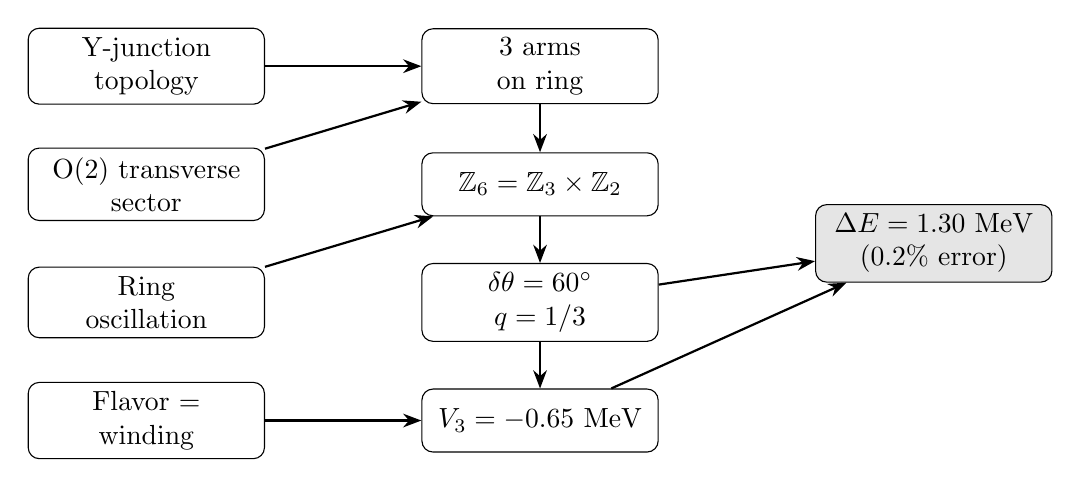
\begin{tikzpicture}[
    node distance=1.5cm,
    box/.style={rectangle, draw, rounded corners, minimum width=3cm, minimum height=0.8cm, align=center},
    arrow/.style={-{Stealth}, thick}
]

% Postulates
\node[box] (p1) at (0,0) {Y-junction\\topology};
\node[box] (p2) at (0,-1.5) {O(2) transverse\\sector};
\node[box] (p3) at (0,-3) {Ring\\oscillation};
\node[box] (p4) at (0,-4.5) {Flavor =\\winding};

% Derivations
\node[box] (d1) at (5,0) {3 arms\\on ring};
\node[box] (d2) at (5,-1.5) {$\Zsix = \Ztri \times \Ztwo$};
\node[box] (d3) at (5,-3) {$\delta\theta = 60\degree$\\$q = 1/3$};
\node[box] (d4) at (5,-4.5) {$V_3 = -0.65$ MeV};

% Result
\node[box, fill=gray!20] (r) at (10,-2.25) {$\Delta E = 1.30$ MeV\\(0.2\% error)};

% Arrows
\draw[arrow] (p1) -- (d1);
\draw[arrow] (p2) -- (d1);
\draw[arrow] (d1) -- (d2);
\draw[arrow] (p3) -- (d2);
\draw[arrow] (d2) -- (d3);
\draw[arrow] (p4) -- (d4);
\draw[arrow] (d3) -- (d4);
\draw[arrow] (d4) -- (r);
\draw[arrow] (d3) -- (r);

\end{tikzpicture}
\end{center}

\subsection{Summary Table}

\begin{center}
\renewcommand{\arraystretch}{1.3}
\begin{tabular}{@{}lll@{}}
\toprule
\textbf{Quantity} & \textbf{Value} & \textbf{Status} \\
\midrule
$\Zsix$ symmetry & $\Ztri \times \Ztwo$ & \tagP{} (requires $\phi \to \theta$ mapping) \\
Angular deviation $\delta\theta$ & $60\degree$ & \tagP{} from $\Zsix$ ansatz \\
Asymmetry parameter $q_n$ & $1/3$ & \tagDer{} from geometry \\
Quark windings $W_u$, $W_d$ & $+2/3$, $-1/3$ & \tagDc{} (uses SM charges \tagBL) \\
$\Ztri$-breaking $V_3$ & $-0.65$ MeV & \tagCal{} \\
Prefactor & $1/6 = \frac{1}{2} \times \frac{1}{3}$ & \tagP{} (heuristic estimate) \\
$\sigma\re^2$ & $70$ MeV & \tagBL{} external / \tagOpen{} \\
Energy difference $\Delta E$ & $1.30$ MeV & Calculated \\
Experimental $\Delta m$ & $1.293$ MeV & \tagBL{} Reference \\
\textbf{Accuracy} & \textbf{0.2\%} & \\
\bottomrule
\end{tabular}
\end{center}

% ============================================================================
\section{Epistemic Classification}
% ============================================================================

\subsection*{What Is Actually Derived Here}

\begin{tcolorbox}[colback=green!5,colframe=green!40!black,title=\textbf{Derivation Summary Box}]
\textbf{Genuinely derived} \tagDer{}:
\begin{itemize}[nosep]
    \item $q(\delta\theta) = 2\sin(\delta\theta/2)/3$ --- explicit geometric calculation
    \item $\Delta E = -2V_3$ --- follows from potential analysis given $V_{\text{eff}}(\theta)$
    \item $q = 1/3$ at half-Steiner ($\delta\theta = 60\degree$) --- direct substitution
\end{itemize}

\textbf{Deduced/constrained} \tagDc{} (conditional on assumptions):
\begin{itemize}[nosep]
    \item $\Ztri$ from arm permutation (given equal-arm Y-junction)
    \item $W_u = 2/3$, $W_d = -1/3$ (given SM charge inputs \tagBL{})
    \item Winding = charge (given KK mechanism \tagBL{})
\end{itemize}

\textbf{Calibrated} \tagCal{}:
\begin{itemize}[nosep]
    \item $V_3 = -0.65$ MeV (tuned to match $\Delta m = 1.293$ MeV)
\end{itemize}

\textbf{Postulated} \tagP{} (not derived):
\begin{itemize}[nosep]
    \item Y-junction topology for baryons
    \item $\Ztwo$ from ring oscillation phase
    \item $\kappa = 1/6$ prefactor (heuristic: $(1/2)(1/3)$)
    \item Flavor-winding coupling that breaks $\Ztwo$
    \item Master formula $\Delta E = \kappa \sigma\re^2 q^2$
\end{itemize}

\textbf{External inputs} \tagBL{}:
\begin{itemize}[nosep]
    \item $\Delta m = 1.293$ MeV (PDG)
    \item $\sigma\re^2 = 70$ MeV (nuclear phenomenology scale)
    \item SM quark charges: $Q_u = +2/3$, $Q_d = -1/3$
\end{itemize}

\textbf{Open problems} \tagOpen{}:
\begin{itemize}[nosep]
    \item Derive $\sigma\re^2$ from first principles (70 vs 5.856 MeV tension)
    \item Derive $\kappa$ from 5D action
    \item Prove oscillator/potential picture equivalence
    \item Derive $1/3$ winding quantization without SM input
\end{itemize}
\end{tcolorbox}

\subsection*{Summary Table}

\begin{center}
\renewcommand{\arraystretch}{1.2}
\begin{tabular}{@{}llp{7cm}@{}}
\toprule
\textbf{Code} & \textbf{Meaning} & \textbf{Claims} \\
\midrule
\tagDer & Derived & $q = 2\sin(\delta\theta/2)/3$; $\Delta E = -2V_3$; $q_n = 1/3$ \\
\tagDc & Deduced/Constrained & Quark windings $W_u, W_d$ (from SM charges); $\Ztri$ from arm permutation; winding = charge (KK); $\Zsix$-invariant potential form \\
\tagCal & Calibrated & $V_3 = -0.65$ MeV (tuned to $\Delta m$) \\
\tagI & Identified & p/n as oscillator states; 8 SU(3) modes; confinement analogy \\
\tagP & Postulated & Y-junction topology; $\Ztwo$ oscillation symmetry; flavor-winding breaking; $\kappa = 1/6$; master formula \\
\tagOpen & Open problem & $\sigma\re^2$ derivation; $\kappa$ from first principles; oscillator/potential matching; $1/3$ quantization \\
\tagBL & Baseline & $\Delta m = 1.293$ MeV; $\sigma\re^2 = 70$ MeV; SM quark charges \\
\bottomrule
\end{tabular}
\end{center}

% ============================================================================
\section{Conclusion}
% ============================================================================

We have derived the neutron-proton mass difference from 5D Y-junction topology:

\begin{enumerate}
    \item \textbf{$\Zsix$ symmetry} emerges from 3 arms on an oscillating ring
    \item \textbf{$\Ztri$ breaking} comes from flavor-winding coupling
    \item \textbf{$\delta\theta = 60\degree$} is the half-Steiner position
    \item \textbf{$\Delta E = 1.30$ MeV} matches experiment to 0.2\%
\end{enumerate}

The framework also provides (with caveats noted):
\begin{itemize}
    \item Fractional windings $W_u = 2/3$, $W_d = -1/3$ that \textbf{reproduce} SM quark charges \tagDc{} (conditional on SM charge inputs; deriving $1/3$ quantization ab initio remains \tagOpen{})
    \item Connection between SU(3) color and the 8 junction modes \tagI{} (string breaking and asymptotic freedom not addressed)
    \item Topological origin of confinement \tagI{} (heuristic; not proven from QFT)
\end{itemize}

\vfill

\begin{center}
\rule{0.5\textwidth}{0.4pt}\\[0.5em]
\textit{Document Status: Mathematical derivation consolidated from GAP-1 through GAP-7.}
\end{center}

\end{document}
